% !TeX root = ../main.tex
% 原始章节：12-fpga-verification.Rmd

\chapter{FPGA上板验证}\label{chap:12-fpga-verification}

\section{基于百芯计划实验箱的基本功能验证}\label{sec:12-fpga-verification-001}

\subsection{实验箱介绍}\label{sec:12-fpga-verification-002}

龙芯``百芯计划''处理器芯片全流程设计，自底向下包括：IP核结构设计、SoC芯片结构设计、芯片后端物理设计、芯片流片封装、硅后系统验证、应用系统开发。各参与高校可根据自身需求参与部分或全部流程的设计。其中IP核结构设计部分，龙芯将会提供参考处理器核设计，处理器核的验证环境与测试用例，合作高校可以进行处理核结构设计与验证或加速器结构设计与验证等。SoC芯片结构设计部分，龙芯将会提供成套外围IP的代码，各接口的驱动程序，专用FPGA设计实验平台，合作高校可以在SoC中IP集成与系统级验证（FPGA）等。芯片后端物理设计部分，龙芯将会提供物理设计参考设计flow，核外部分的GDS，合作高校可以进行全芯片物理设计或IP核物理设计等。硅后系统验证部分，龙芯将会提供开发板设计参考，合作高校可以在开发板对芯片各功能进行系统调试与验证等。应用系统开发部分，合作高校可以基于芯片研制具体问题的解决方案等。

板卡在原有基础上去掉板载NAND颗粒，改成TF卡槽，方便大容量存储拓展；增加SDRAM颗粒，方便学生使用SDRAM方案进行设计，容量增加到2Gb（删除原有的SRAM）；USB接口方案进行更换，接口拓展为4个，增加了更多外设的兼容；现有LCD屏更换为智能串口HMI屏，便于根据需求进行屏幕的个性化设计；增加SPI接口的引出。板卡可以满足百芯计划所需的外设需求，兼容原有的数字逻辑、体系结构、组成原理实验的硬件接口。板载系统资源如图\ref{fig:baixin-arch}所示。

\begin{figure}[htbp]
  \centering
  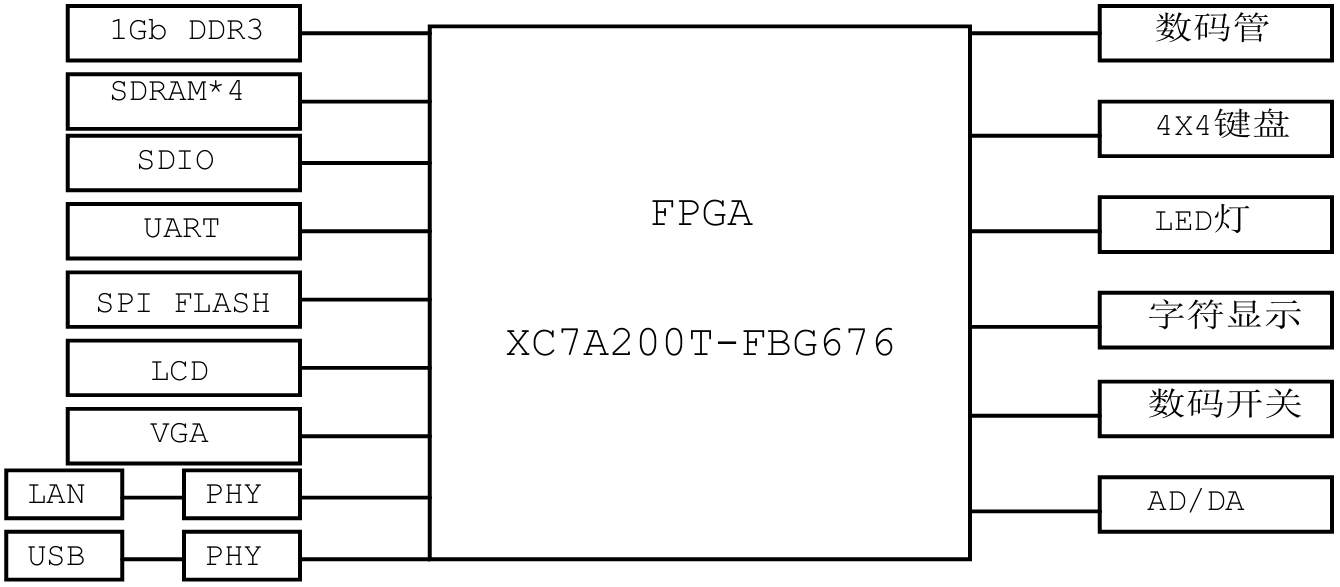
\includegraphics[width=0.75\linewidth]{assets/12/baixin_arch.png}
  \caption{百芯开发板资源}
  \label{fig:baixin-arch}
\end{figure}

\subsection{系统验证 SoC 介绍}\label{sec:12-fpga-verification-003}

龙芯提供的百芯开发板 SoC 位于chplab工程下，相关目录如下

% 代码语言：text
\begin{CodeBlock}
.
├── chip              SoC顶层。
│　　└── soc_demo       SoC顶层代码实例。
│　　　　　├── loongson    龙芯实验箱SoC顶层代码。
│　　　　　├── Baixin      百芯开发板SoC顶层代码。
│　　　　　└── sim       仿真SoC顶层代码
├── fpga              综合工程。
│　　├── loongson        龙芯实验箱综合工程。
│　　　　　├── 2019.2    对应Vivado 2019.2版本。
│　　　　　└── 2023.2    对应Vivado 2023.2版本。
│　　└── Baixin          百芯开发板综合工程。
├── IP                SoC IP。
│　　├── AMBA         总线 IP。
│　　├── APB_DEV       APB协议通信设备。
│　　　　　├── URT       UART设备控制器。
│　　　　　└── NAND     NAND设备控制器。
│　　├── AXI_DELAY_RAND  随机延迟注入。
│　　├── AXI_SRAM_BRIDGE  AXI协议 -> SRAM接口转换。
│　　├── BRIDGE        1x2桥接模块。
│　　├── DMA          DMA逻辑，用于设备作为master访问内存。
│　　├── SPI           SPI Flash设备控制器。
│　　├── MAC          MAC设备控制器。
│　　├── CONFREG       用于访问开发板上数码管、拨码开关等外设以及特殊寄存器。
│　　├── myCPU        处理器核逻辑。
│　　└── xilinx_ip        Vivado平台所创建的IP。
│　　　　　├── 2019.2    对应Vivado 2019.2版本。
│　　　　　└── 2023.2    对应Vivado 2023.2版本。
\end{CodeBlock}

SoC设备及地址空间划分如下：

\begin{longtable}[]{@{}
  >{\raggedright\arraybackslash}p{(\linewidth - 6\tabcolsep) * \real{0.3710}}
  >{\raggedright\arraybackslash}p{(\linewidth - 6\tabcolsep) * \real{0.0645}}
  >{\raggedright\arraybackslash}p{(\linewidth - 6\tabcolsep) * \real{0.3710}}
  >{\raggedright\arraybackslash}p{(\linewidth - 6\tabcolsep) * \real{0.1935}}@{}}
\toprule\noalign{}
\begin{minipage}[b]{\linewidth}\raggedright
地址范围
\end{minipage} & \begin{minipage}[b]{\linewidth}\raggedright
模块
\end{minipage} & \begin{minipage}[b]{\linewidth}\raggedright
描述
\end{minipage} & \begin{minipage}[b]{\linewidth}\raggedright
空间大小
\end{minipage} \\
\midrule\noalign{}
\endhead
\bottomrule\noalign{}
\endlastfoot
0x1C000000 - 0x1C0FFFFF & SPI & SPI 控制器（boot rom） & 1 MB \\
0x1FE80000 - 0x1FE8FFFF & SPI & SPI 控制器 & 64 KB \\
0x1FE00000 - 0x1FE0FFFF & APB & APB\_DEV: UART & 64 KB \\
0x1FE70000 - 0x1FE7FFFF & APB & APB\_DEV: NAND（未使用） & 64 KB \\
0x1FD00000 - 0x1FD0FFFF & CONF & 配置寄存器及GPIO & 64 KB \\
0x1FF00000 - 0x1FF0FFFF & MAC & MAC 控制器 & 64 KB \\
其他 & DDR3 & DDR3 内存 & 依赖具体实现 \\
\end{longtable}

\subsubsection{内核启动的方法}\label{sec:12-fpga-verification-004}

本文以内核启动为例简单介绍一下SoC代码整体的使用流程。

内核启动需要依次完成以下步骤：

\begin{itemize}
\tightlist
\item
  烧写 PMON 文件(\href{https://gitee.com/chenzes/chiplab-tools/releases/download/pmon/gzrom.bin}{gzrom.bin})或 u-boot文件(\href{https://gitee.com/llh730/la32r-uboot/releases}{uboot.bin})到可插拔 SPI flash 上。
\item
  生成并加载 bit 流文件。
\item
  运行 PMON / u-boot。
\item
  搭建 tftp 服务器 Load 内核(\href{https://gitee.com/loongson-edu/la32r-Linux/releases}{vmlinux})。
\item
  启动内核。
\end{itemize}

\textbf{1. 烧写PMON / u-boot}

烧录方面我们推荐使用\href{https://detail.tmall.com/item.htm?spm=a21n57.1.item.2.21e3523cc9elHp\&priceTId=2147bfb717231061625906771e52e0\&utparam=\%7B\%22aplus_abtest\%22\%3A\%22abee490f5aa02657b98af3e8efcc7a9b\%22\%7D\&id=807896685118\&ns=1\&abbucket=10\&xxc=taobaoSearch\&skuId=5659871783574\&pisk=fR8ttPGMuvDMFZnD5Cihow64wxGnEFdZIdR7otXgcpppG94m_NmVkKBp3OjG5O4AkIp2nKdq_s6XhKBDjD0k_C7VlY4xr4AwYwZe1dBbl9Gfa_rjW2mn1C7VlxF3l00J_LhWJmDAcXQCMsZ1lG_bR66FMsw6hOsQd_CPlt9flXQCgsXb5O_bOJ1jCDcF3vXuknOCXJ97-Sz0oeCI3TOTfrCHR1UCeCBKFV8LzGBW19UjE5hM5tBePvmpTLx6I6JxyvQW4pLAVZ3TU1KBww6GPVFNFFfvZnd-e-fefdLCDecqbBLABgT1vqhlRNCXhiKEezfOSHIJWhl4dC9lB3_wi7HM9gKd46sQMl_MqQYVVFgTU9jPMpIkXYU9Fgl6rUEjq8XRilGK9orVf6jlSZz6mdUr36BotGZ40MeO9TcK9orVf65dEX4_0oSLB}{CH341A编程器}烧写 PMON 文件(\href{https://gitee.com/chenzes/chiplab-tools/releases/download/pmon/gzrom.bin}{gzrom.bin})或 u-boot文件(\href{https://gitee.com/llh730/la32r-uboot/releases}{uboot.bin})到开发板搭载的可插拔 SPI flash 上。商家提供的资料比较全面，上位机软件支持图形化界面，使用简单。

\textbf{2. 下载bit流文件}

打开\texttt{chiplab/fpga/Baixin/system\_run/system\_run.xpr}工程综合并生成 bit 流。将开发板与主机间的下载线连接好，开发板上电，使用 Vavidao 工具里的 Open Hardware Manager 下载 bit 文件到开发板上。

\textbf{3. 运行PMON / u-boot}

上述烧写的 PMON / u-boot 运行在下载的 SoC 上，需要使用串口展示运行信息。 将开发板与主机间的串口线连接好，打开串口软件，波特率设置为 115200。

Windows下可以使用免安装的\href{https://gitee.com/chenzes/chiplab-tools/releases/download/chiplab-tools/SecureCRTPortable.zip}{SecureCRTPortable串口软件}。 先使用 USB 转串口和串口连接线将电脑和开发板相连。
双击程序打开，第一次启动界面如下图\ref{fig:secure-one}所示：

\begin{figure}[htbp]
  \centering
  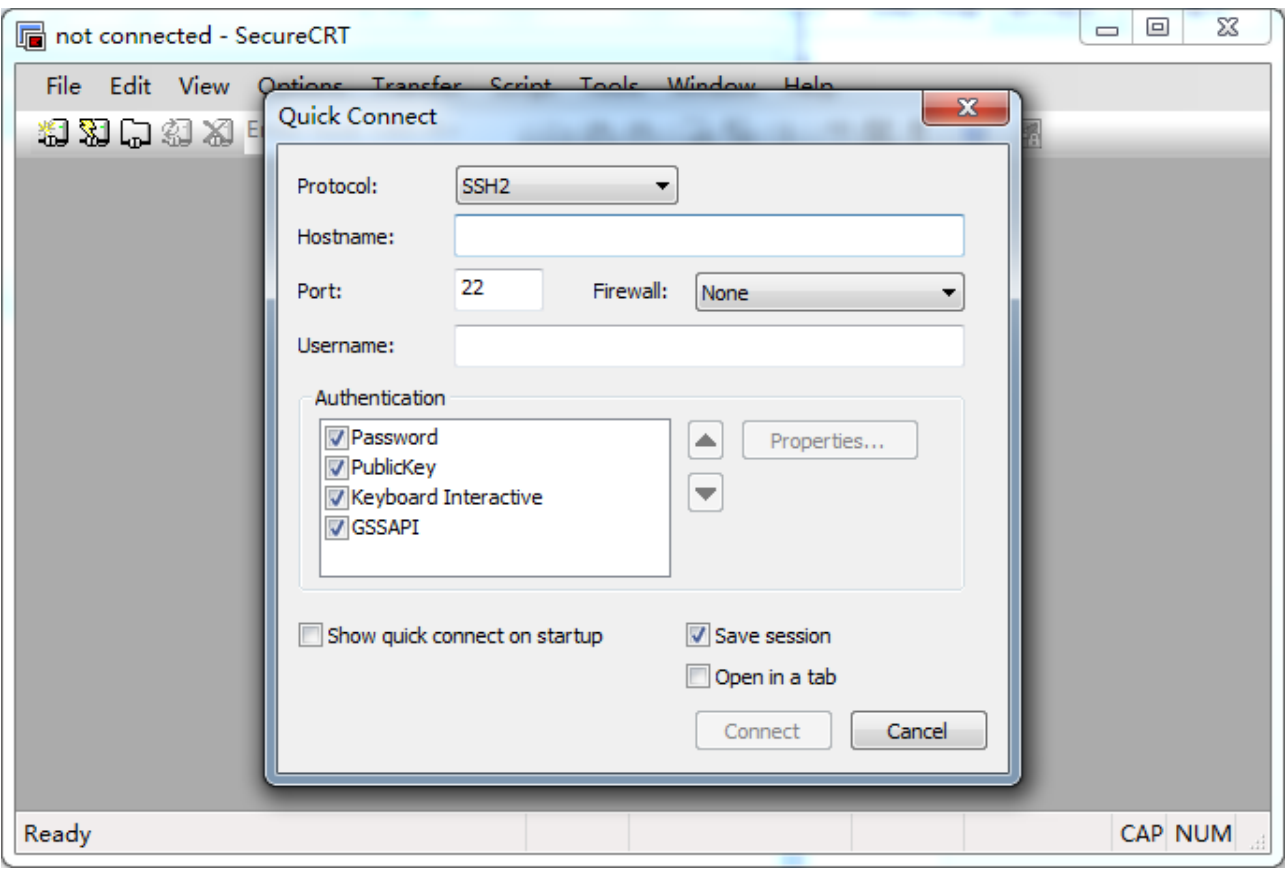
\includegraphics[width=0.75\linewidth]{assets/12/secure_one.png}
  \caption{启动界面}
  \label{fig:secure-one}
\end{figure}

第一行 Protocol 下拉选择 Serial，如下图\ref{fig:secure-two}所示：

\begin{figure}[htbp]
  \centering
  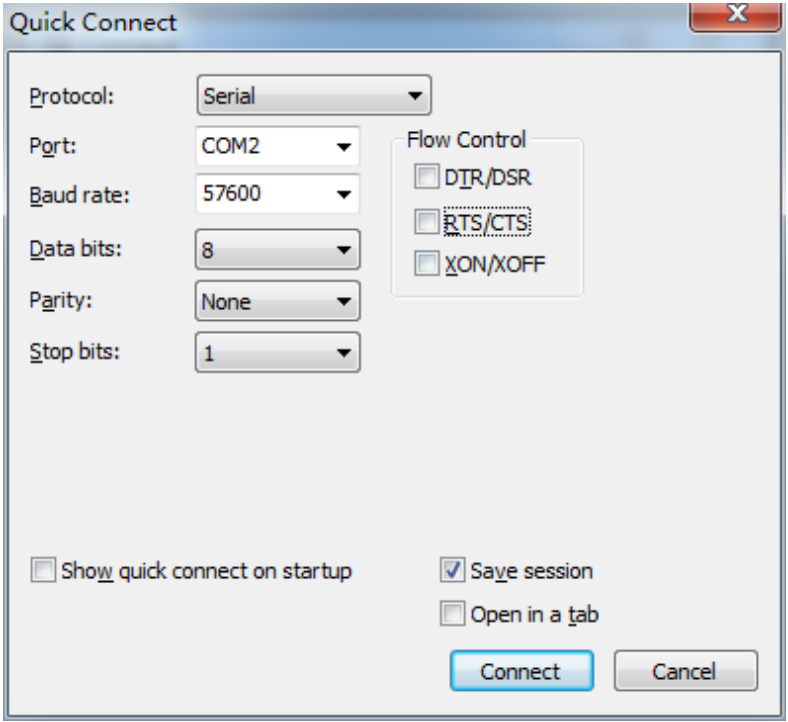
\includegraphics[width=0.75\linewidth]{assets/12/secure_two.png}
  \caption{选择串口}
  \label{fig:secure-two}
\end{figure}

其中 Baud rate 为选择波特率，需根据开发板上串口控制器的初始化代码中设置的波特率进行选择(对于本次校验设备，波特率需选择 115200)。右侧 Flow Control 全不选。Port 的选择需根据 Windows 电脑上的端口进行选择，可以右键电脑选择设备管理器进入设备管理器查看，如下图\ref{fig:secure-three}所示：

\begin{figure}[htbp]
  \centering
  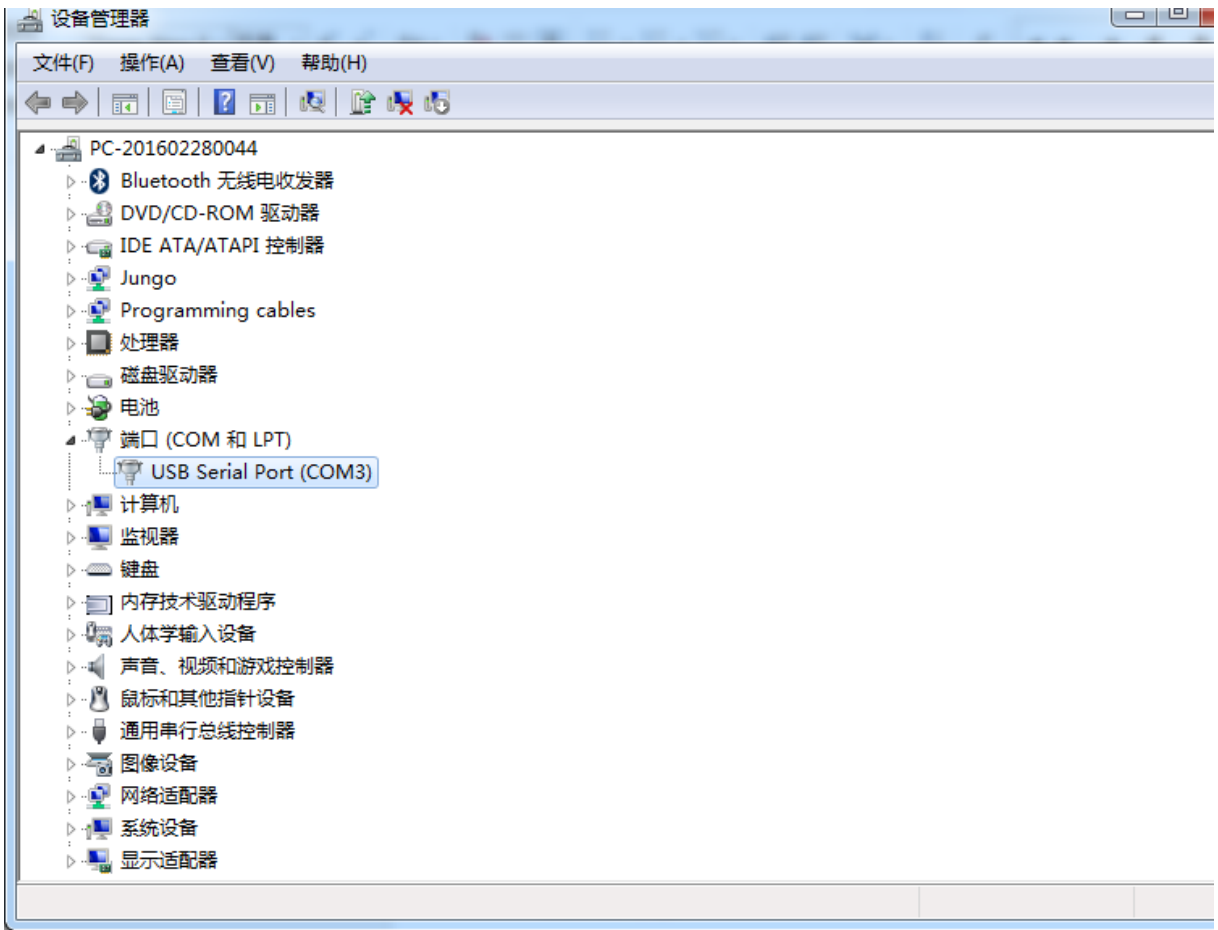
\includegraphics[width=0.75\linewidth]{assets/12/secure_three.png}
  \caption{配置串口}
  \label{fig:secure-three}
\end{figure}

配置好串口后，点击 connect，即可进入串口界面，在波特率设置正确的情况下，可以通过串口与开发板进行交互，如下图\ref{fig:secure-four}所示：

\begin{figure}[htbp]
  \centering
  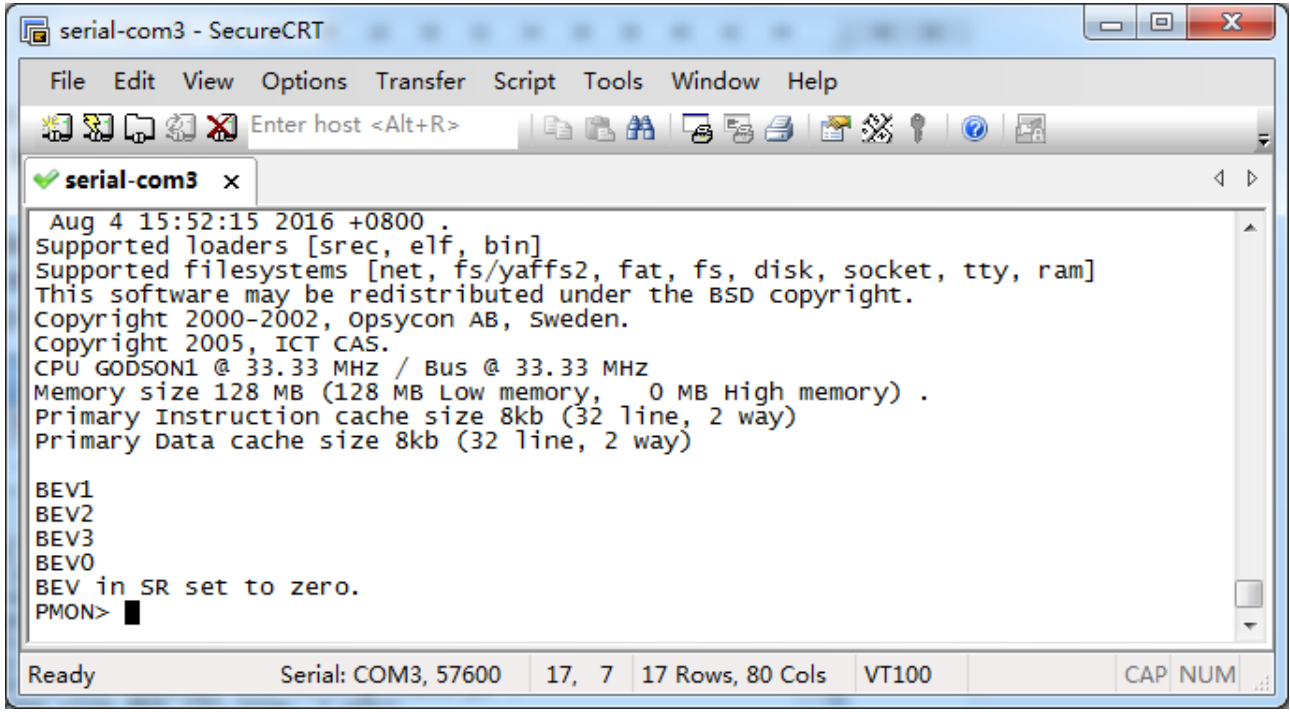
\includegraphics[width=0.75\linewidth]{assets/12/secure_four.png}
  \caption{成功连接串口}
  \label{fig:secure-four}
\end{figure}

\textbf{4. PMNO网络加载并运行Linux}

连接上串口，打开串口软件，设置好波特率，则可以在串口窗口中看到 PMON 运行信息，运行成功后则会进入 PMON 提示符，此时可以输入 PMON 命令。

比如， SoC 中具有 MAC 控制器，PMON 中也有 MAC 驱动，则我们输入命令

% 代码语言：text
\begin{CodeBlock}
ifconfig dmfe0 10.90.50.44
\end{CodeBlock}

则可以给开发板上的网卡配置 IP 为 10.90.50.44（具体需配置的 IP 请查阅同网段的电脑 IP），假设同网段的电脑 IP 为 10.90.50.43,则可以继续输入命令

% 代码语言：text
\begin{CodeBlock}
ping 10.90.50.43
\end{CodeBlock}

用于查看网络是否成功接入。Linux 在 ping 网络是会一直发 ping 包，可以 \texttt{Ctrl+C} 取消 ping。运行结果如下：

% 代码语言：text
\begin{CodeBlock}
PMON> ifconfig dmfe0 10.90.50.44
rx ring 70acee0
tx ring 70acf60
DE4X5_BMR= fe000000
DE4X5_TPD= 0
DE4X5_RRBA= 70acee0
DE4X5_TRBA= 70acf60
DE4X5_STS= f0660004
DE4X5_OMR= 32002242
TX error status2 = 0x00000000
After setup
DE4X5_BMR= fe000000
DE4X5_TPD= 0
DE4X5_RRBA= 70acee0
DE4X5_TRBA= 70acf60
DE4X5_STS= f0660004
DE4X5_OMR= 32002242
PMON> ping 10.90.50.43
PING 10.90.50.43 (10.90.50.43): 56 data bytes
64 bytes from 10.90.50.43: icmp_seq=0 ttl=64 time=3.708 ms
64 bytes from 10.90.50.43: icmp_seq=1 ttl=64 time=2.331 ms
64 bytes from 10.90.50.43: icmp_seq=2 ttl=64 time=2.235 ms

--- 10.90.50.43 ping statistics ---
3 packets transmitted, 3 packets received, 0% packet loss
round-trip min/avg/max = 2.235/2.750/3.708 ms
PMON>
\end{CodeBlock}

由于运行 linux 时，最初的内核需要使用网口 load 进入内存执行，因而需要先搭建 Tftp 服务器。
具体方法参见\href{https://gitee.com/chenzes/chiplab-tools/releases/download/chiplab-tools/tftp.zip}{tftp下载地址}。
目前运行 Linux 的方法是，先运行 PMON，随后通过网口 load Linux 内核进入 FPGA 上的 DDR3 内存上。在load内核前，需要通过以下命令裁剪掉内核二进制文件中的符号信息。

% 代码语言：text
\begin{CodeBlock}
loongarch32r-linux-gnusf-strip vmlinux
\end{CodeBlock}

load 命令为

% 代码语言：text
\begin{CodeBlock}
load tftp://10.90.50.43/vmlinux
\end{CodeBlock}

其中 10.90.50.43 为搭建的 tftp 服务器的 IP。
串口的波特率为 115200。
具体过程如下：
启动 PMON 后，输入命令

% 代码语言：text
\begin{CodeBlock}
ifconfig dmfe0 10.90.50.44
\end{CodeBlock}

给开发板上的网卡配置 IP 为 10.90.50.44（具体需 配置的 IP 请查阅同网段的电脑 IP），假设同网段的电脑 IP 为 10.90.50.43, 则可以继续输入命令

% 代码语言：text
\begin{CodeBlock}
ping 10.90.50.43
\end{CodeBlock}

用于查看网络是否成功接入。
网络配置好了，需要通过网络下载 Linux 内核，需要先搭建好 tftp 服务器，假设搭建的 tftp 服务器 IP 为 10.90.50.43，将要下载 Linux 内核放到 tftp 服务器的根目录下，输入命令

% 代码语言：text
\begin{CodeBlock}
load tftp://10.90.50.43/vmlinux
\end{CodeBlock}

即可 load 内核进入 FPGA 上的内存。

% 代码语言：text
\begin{CodeBlock}
PMON> load tftp://10.90.50.43/vmlinux
Loading file: tftp://10.90.50.43/vmlinux (elf)
0x80200000/5350380 + 0x8071a3ec/169220(z) + 6926 syms\
Entry address is 802041f0
PMON> g console=ttyS0,115200 rdinit=sbin/init
\end{CodeBlock}

上表中显示 load 成功了，输入命令

% 代码语言：text
\begin{CodeBlock}
g console=ttyS0,baudrate rdinit=sbin/init
\end{CodeBlock}

即可运行该内核，命令中 baudrate 需为数字，即为串口控制器设置的波特率，设置不对时，串口显示字符为乱码。Linux 内核运行时波特率为 115200。
当运行 Linux 内核成功后会出现\texttt{/\ \#}提示符，可以使用常用的 Linux 命令。

\textbf{4. U-Boot网络加载并运行Linux}

连接上串口，打开串口软件，设置好波特率，则可以在串口窗口中看到 u-boot 运行信息，运行成功后则会进入 u-boot 提示符，此时可以输入 u-boot 命令。

在u-boot中使用\texttt{print}命令可以查看当前的环境配置。

使用命令（\textbf{请使用自己的IP}）

% 代码语言：text
\begin{CodeBlock}
setenv ipaddr 10.90.50.44
setenv serverip 10.90.50.43
\end{CodeBlock}

可以配置u-boot和服务器（自己电脑）的使用的ip（两者需在同一子网下，配置的具体IP需查看自己本机IP），u-boot中通过命令

% 代码语言：text
\begin{CodeBlock}
ping 10.90.50.43
\end{CodeBlock}

可以查看与服务器是否建立了连接。

完成了网络配置，就可以使用uboot加载内核，使用命令

% 代码语言：text
\begin{CodeBlock}
setenv bootcmd console=ttyS0,115200 rdinit=/init
\end{CodeBlock}

可以配置内核的启动参数。 通过命令

% 代码语言：text
\begin{CodeBlock}
tftpboot 0xa3000000 vmlinux
\end{CodeBlock}

可以将内核加载到 \texttt{0xa300\_0000} 开始的地址上，该地址并不是\texttt{readelf}显示的\texttt{entry}的入口地址。uboot会先把镜像加载到一段无数据的地址，运行时再根据elf段的信息加载到对应的位置上。

最后，使用命令

% 代码语言：text
\begin{CodeBlock}
bootelf 0xa3000000 bootcmd
\end{CodeBlock}

即可成功运行linux内核！

\section{设计包含各类外设的测试板}\label{sec:12-fpga-verification-005}

如果现有的开发板资源不满足我们的开发需求，我们可自行设计验证板（包括FPGA测试板和回片测试板）、板载集成支持各类外设配套的控制器、转接口、IO调试等资源，以完整验证CPU功能、操作系统与应用程序验证演示。但是PCB电路设计相关知识和注意事项并不是本文关注的重点，这里仅对一些常见且必要的设备做简单介绍。在实践流程文档中，我们将以LainBoard为例，介绍测试板的设计。

\subsection{DRAM控制器}\label{sec:12-fpga-verification-006}

DRAM内存是整个SoC的主存储器，在整个SoC中占有最重要的地位，其容量决定了CPU处理大量数据的能力大小，而其速率决定了CPU处理数据的快慢。同时，如果DRAM控制器不工作，则在选定SDRAM内存是1990年代的技术，速度较慢，但其接口简单，没有复杂的时序要求，且芯片廉价易购买。SDRAM具有由时钟驱动的同步传输接口，只需要使用简单的IOPAD及开源的控制器IP核就可驱动，而如果使用DDR内存，则需要增加Interface PHY IP核和控制器，增加设计的复杂程度。一般考虑项目的实际情况，最适宜的内存类型就是SDRAM内存。

\subsection{SPI Flash控制器}\label{sec:12-fpga-verification-007}

SPI Flash控制器通过SPI总线接口连接到芯片外部的SPI Flash总线，对内具有AXI接口，将AXI接口上的访存请求翻译为SPI Flash控制指令，然后从Flash存储芯片中读出数据并在AXI接口上返回。CPU核心启动时的PC地址对应SPI Flash存储区域，开机时CPU即可通过直接访存的形式读取Bootloader代码并执行。使用SPI Flash存放启动代码的好处是可以使启动代码在芯片设计结束后随时可修改，避免在芯片内部使用ROM固化的代码中存在Bug的情况。SPI Flash控制器也兼具SPI控制器的作用，可以连接SPI LCD显示屏等外设，并进行高速双向通信。对应的，测试板上可搭载Flash芯片或引出SPI接口。

\subsection{以太网控制器}\label{sec:12-fpga-verification-008}

网络通信是计算机系统的重要能力。以太网接口控制器分为两部分：MAC和PHY，前者为逻辑控制器，很容易放进芯片中；后者为物理层接口，一般需要模拟电路来实现，两者之前采用MII或RMII接口相连{[}27{]}。在芯片中具有AXI接口的以太网控制器，该控制器支持10/100Mbps的通信速率，与外部以MII总线相连，并外接了MII转RMII转换器，对外暴露RMII接口。

以太网控制器分为总线、网络两个时钟域，总线时钟域负责与CPU进行通信，网络时钟域负责与MII接口进行通信，两个模块之间通过CDC同步器进行沟通。以太网控制器模块内具有四个双端口SRAM存储器，每个存储器的两个端口分别连接到两个时钟域。在发送数据包时，首先在总线时钟域侧由CPU将数据写入SRAM，然后网络时钟域侧的逻辑将SRAM内容搬运到MII接口；接收数据包时，在网络时钟域侧从MII接口将数据包内容搬运到SRAM，再由CPU向总线时钟域侧的逻辑读取。

MII是控制器与PHY的中间数字接口，并不是最终连接以太网的接口。芯片要与实际的以太网接口相连，还需要PHY芯片将数字接口适配以太网接口的物理定义。

\subsection{SD卡控制器}\label{sec:12-fpga-verification-009}

现代操作系统通常需要磁盘的支持，用于存放程序、资源文件、用户文件等。主流计算机磁盘的接口有IDE、SATA、NVMe等，但这些接口（特别是后两者）都较为复杂，在短时间内集成进本芯片是不现实的。SD卡作为近年来新兴的存储设备，具有简单的协议和接口，且容量大、价格低廉、容易购买，适合作为测试板的存储设备使用。

\subsection{I2C控制器}\label{sec:12-fpga-verification-010}

I2C（全称Inter-Integrated Circuit）是Philips公司于1982年提出的一种通讯总线，使用两条线就可以连接多个外设，使PCB设计变得更加简单方便。I2C总线通常用于连接低速外设，如各种传感器。

\subsection{UART控制器}\label{sec:12-fpga-verification-011}

UART控制器使芯片可以通过UART协议（串口）与外部进行通信。龙芯教育提供了一个标准的16550 UART控制器，挂接到APB总线下。UART控制器中有FIFO功能，CPU可以一次性写入多组数据，加快通信速率。

\subsection{USB控制器}\label{sec:12-fpga-verification-012}

USB（通用串行总线）是一种广泛使用的设备接口，用于连接电脑和其他电子设备。它允许设备之间的数据传输，并可以为连接的设备供电。一般来说在SoC中会继承支持ULPI接口的USB控制器，而开发板则需要搭载USB PHY芯片以支持USB通信。

\subsection{小结}\label{sec:12-fpga-verification-013}

总的来说我们的测试板一般需要搭载如下设备：

\begin{enumerate}
\def\labelenumi{\arabic{enumi}.}
\tightlist
\item
  电源控制芯片
\item
  SDRAM内存芯片
\item
  Flash闪存芯片
\item
  以太网PHY芯片和RJ45网口
\item
  USB PHY芯片及USB母座
\item
  SD卡插槽
\item
  SPI、GPIO、I2C等信号接口排母
\item
  按需求添加的其他设备
\end{enumerate}
